\chapter{Элементы, которые могут присутствовать в тексте}

\section{Формулы}

Для оформления формул и уравнений используются стандартные возможности \LaTeX.
Выключные формулы должна быть оформлены как окружение \verb|equation|.
Пояснения символов и числовых коэффициентов, входящих в формулу, если они не
пояснены ранее в тексте, должны быть приведены непосредственно под формулой.
Пояснение каждого символа следует давать в той последовательности, в которой
символы приведены в формуле. Первая строка пояснения должна начинаться
со слова  <<где>> без двоеточия после него. Формулы, следующие одна за другой
и не разделенные текстом, разделяют запятой

Ниже приведен простейший пример
\begin{equation}\label{eq:H0}
H_0 = \frac{p^2}{2 m} + a_0\, x^4 - a_2\, x^2,
\end{equation}
где  $p$ "--- импульс частицы, $m$ "--- масса частицы, $x$ "--- координата
частицы, $a_0, a_2$ "--- параметры системы.

Нумерация формул осуществляется автоматически в пределах главы, как это
продемонстрировано для формулы~\eqref{eq:H0}. Переносить формулы на следующую
строку допускается только на знаках выполняемых операций, причем знак в начале
следующей строки повторяют. 

Ссылки в тексте на порядковые номера формул дают в скобках, например:
в формуле~\eqref{eq:H0}.

А это уже более сложный пример
\begin{align}
H^0_{m\, n} & = \delta_{m + 4 \; n} \;
\frac{a_0 g^2}{4} \sqrt{(m + 1)(m + 2)(m + 3)(m + 4)} +\notag\\
& + \delta_{m + 2 \; n} \;
\frac{g}{2} a_0  (2 m + 3) \sqrt{(m + 1)(m  + 2)}.\label{eq:Hmn}
\end{align}
где $g = \frac{m}{a_0}$ "--- числовой коэффициент, или так:
$\displaystyle{g = \frac{m}{a_0}}$, если поместить внутристрочную формулу
в аргумент команды \verb|\displaystyle{}|.



\section{Рисунки}

Для вставки рисунков рекомендуется использовать пакеты graphics или graphicx
и команду \verb|\includegraphics|. Рисунок оформляется с использованием
стандартного окружения \verb|figure|, которое обеспечивает его автоматическую
нумерацию. Рисунок и подпись вставляются при помощи стандартных команд
\verb|\includegraphics| и \verb|\caption{Подпись}|, соответственно.
Подрисуночная подпись должна пояснять что изображено на рисунке, также может
содержать уточняющую информацию. 

Рисунки должны быть пронумерованы и иметь подпись, которая всегда должна
располагаться  под рисунками. Рисунки могут быть представлены в форматах
*.pdf, *.ps, *.eps, *.jpg,  *.png или *.tif и должны иметь разрешение не
менее 300 dpi. 

Убедитесь, что линии на рисунках не прерываются и имеют постоянную ширину.
Сетки и детали на рисунках должны быть четкими и не должны быть начертаны
друг на друге. Аббревиатуры, используемые на рисунке, должны быть определены
в тексте отчета, если они не являются общими сокращениями или уже были
определены в тексте. Легенда должна пояснять все используемые символы и
должна входить с состав рисунке, а не содержаться в словесных пояснениях
в подписях (например, <<пунктирная линия>> или <<открытые зеленые кружки>>).

На все рисунки в тексте должна быть ссылка до появления самого рисунка в
тексте отчета, например: рисунки \ref{fig:01}, \ref{fig:02}.

\begin{figure}[h!]
\begin{center}
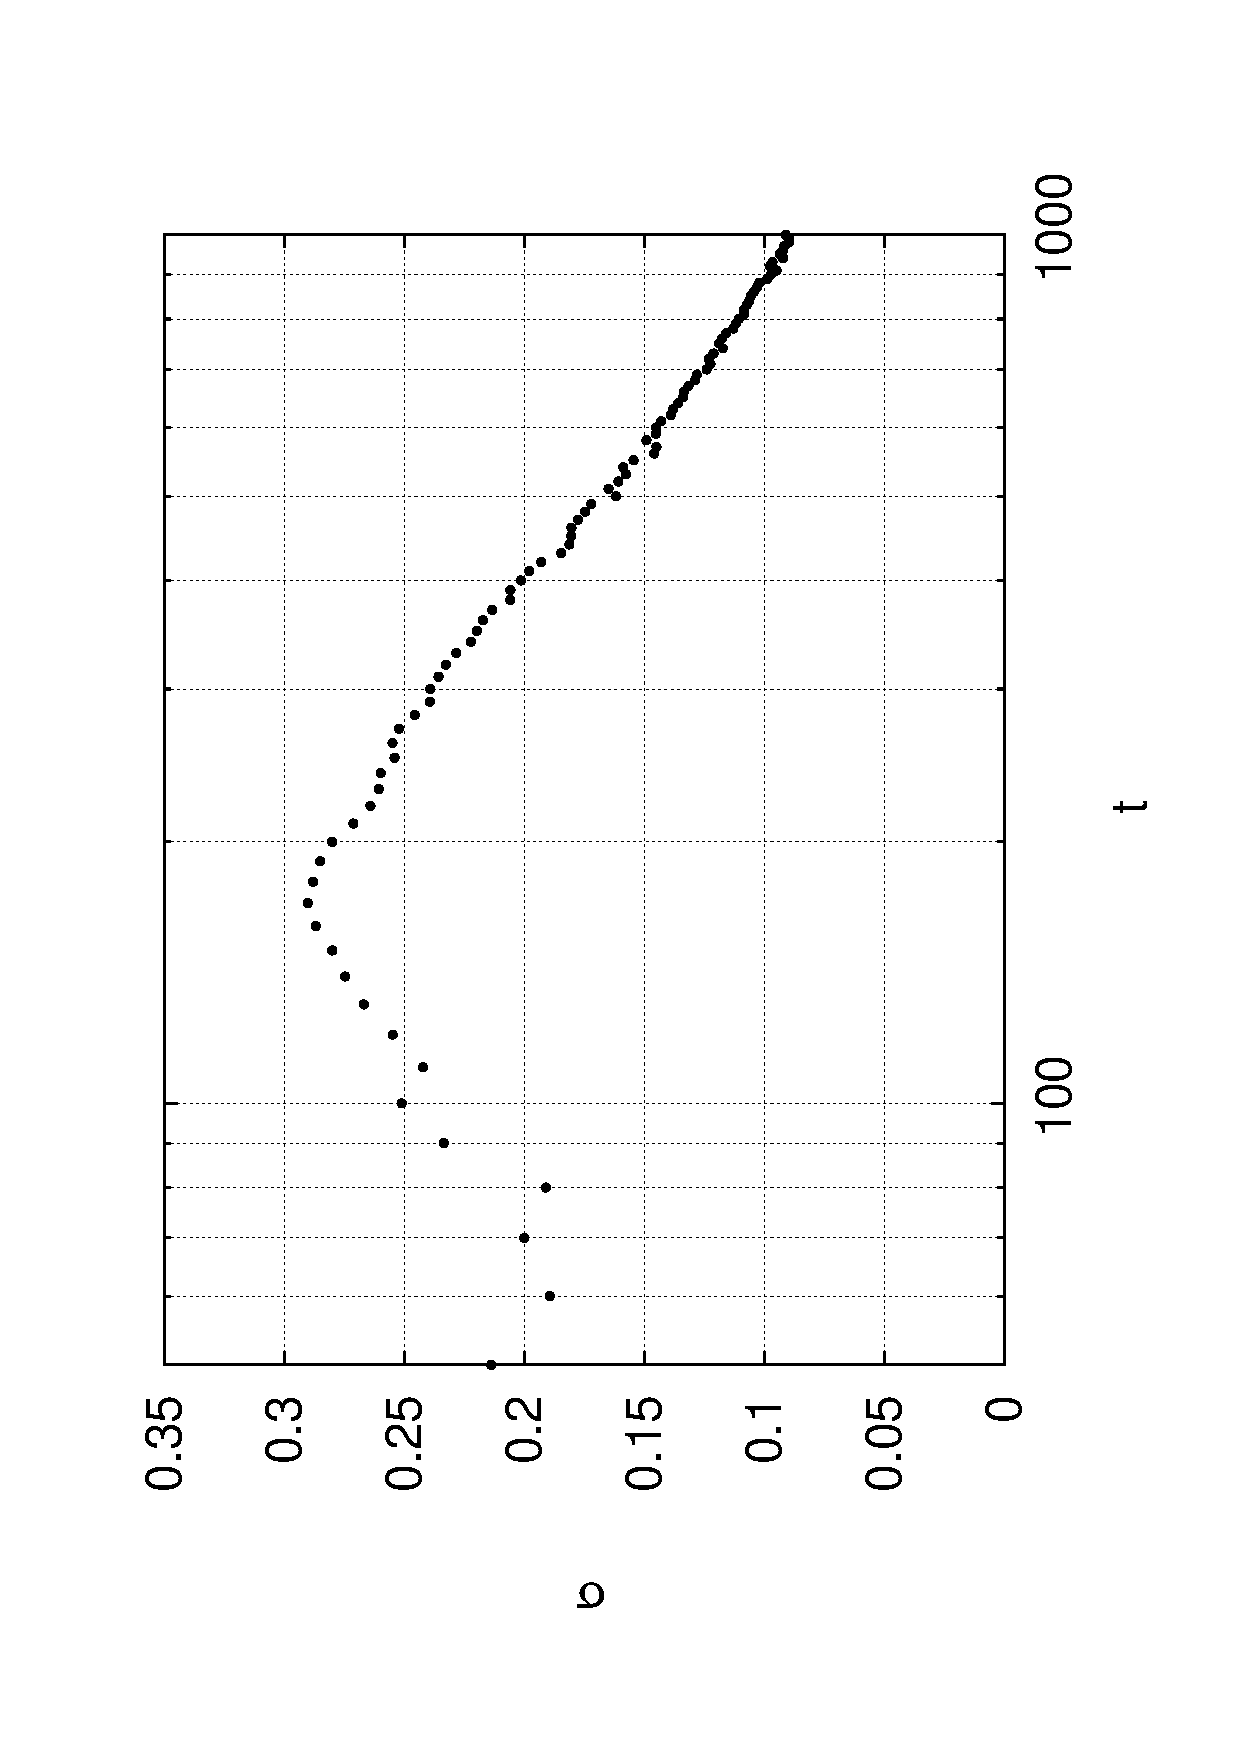
\includegraphics[angle=270,width=10cm]{test}\\[2mm]
\caption{Подпись к рисунку. Дополнительная информация. Дополнительная инофрмация}
\label{fig:01}
\end{center}
\end{figure}

\begin{figure}[h!]
\begin{center}

\includegraphics[width=0.5\hsize]{empty.jpg}\\[2mm]
\caption{Пример использования *.jpg}
\label{fig:02}
\end{center}
\end{figure}

Если возникает необходимость привести в тексте рисунок, который не помещается
на одной странице, например, это может быть большая блок-схема, то номер
рисунка не должен изменяться, а в конце подписи к нему должно быть указано:
Лист~1. На следующей странице должен быть приведен только номер рисунка,
а подпись должна содержать только Лист~2.
Например: Рисунок~2.1 "--- Лист~2.


\section{Таблицы}

Для создания таблиц используется окружение \verb|table|, которое обеспечивает
нумерацию и создание заголовка. Для помещения заголовка над
таблицей в начале указанного окружения необходимо задать команду
\verb|\capition{Подпись к таблице}|. Сама таблица может оформляться с помощью
стандартного окружения \verb|tabular|. Пример таблицы приведен ниже (таблица~\ref{tab:1}). 

\begin{table}[h]
\caption{Название таблицы. Таблицы следует размещать в основном тексте рядом с первым цитированием.}
\label{tab:1}
\begin{center}
\begin{tabular}{|l|c|c|}
\hline
Заголовок 1 & Заголовок 2 & Заголовок 3 \\
\hline
Запись 1 &данные &данные\\
\hline
Запись 2 &данные &данные\\
\hline
Запись 3 &данные &данные\\
\hline
\end{tabular}
\end{center}
\end{table}

На все таблицы документа должны быть приведены ссылки в тексте
документа до появления самой таблицы. При ссылке следует писать слово
<<таблица>> с указанием её номера.

В случае наличия в тексте длинных таблиц, которые не помещаются на одной
странице, необходимо использовать окружение \verb|longtable|.

\section{Листинги программ}

Листинги программ могут быть расположены как в тексте отчета (возможно ближе к 
соответствующим частям текста, содержащим ссылку на листинг),  так и в конце
его текста отчета (в приложениях). Листинг, за исключением листингов
приложений, следует нумеровать арабскими цифрами с нумерацией в пределах главы
(листинг~\ref{ls:01}).
Листинг каждого приложения обозначают отдельной нумерацией арабскими цифрами с
добавлением перед цифрой обозначения приложения.
Например: Листинг~\ref{ls:a:01}.
На все листинги должны быть ссылки в тексте отчета до появления самого
листинга, примеры таких ссылок приведены выше.

\begin{lstlisting}[caption={Пример листинга в тексте}, label={ls:01}]
// a simple kernel that simply increments each array element by b
__global__ void kernelAddConstant(int *g_a, const int b) {
  int idx = blockIdx.x * blockDim.x + threadIdx.x;
  g_a[idx] += b;
}
\end{lstlisting}
